\chapter{Score Calibration Analysis}
\label{chap:score_calibration}
\section{Calibration Results (K-Fold Validation)}
To address the severe calibration losses observed at extreme priors, we applied a score calibration transformation. The calibration mapping was learned using a prior-weighted Logistic Regression trained via a 5-fold cross-validation strategy on the validation scores to prevent optimistic bias.
Table \ref{tab:calibrated_results} presents the Minimum DCF and Actual DCF of the calibrated models compared against their raw, uncalibrated Actual DCF, systematically grouped by model architecture to observe performance across the three target applications.
\begin{table}[H]
\centering
\caption{Performance of Calibrated Models (K-Fold Validation) vs. Raw Actual DCF, grouped by Model.}
\label{tab:calibrated_results}
\resizebox{\textwidth}{!}{
\begin{tabular}{llccc}
\toprule
\textbf{Model} & \textbf{Application Prior ($\tilde{\pi}$)} & \textbf{Raw Act. DCF} & \textbf{Calibrated Act. DCF} & \textbf{Calibrated Min DCF} \\
\midrule
\multirow{3}{*}{\textbf{Logistic Regression}}
& 0.1 & 0.413 & \textbf{0.387} & 0.372 \\
& 0.5 & 0.187 & \textbf{0.185} & 0.181 \\
& 0.9 & 0.471 & \textbf{0.462} & 0.444 \\
\midrule
\multirow{3}{*}{\textbf{SVM (RBF)}}
& 0.1 & 0.631 & \textbf{0.347} & 0.319 \\
& 0.5 & 0.159 & \textbf{0.158} & 0.151 \\
& 0.9 & 0.694 & \textbf{0.411} & 0.397 \\
\midrule
\multirow{3}{*}{\textbf{GMM (Tied)}}
& 0.1 & 0.303 & \textbf{0.279} & 0.265 \\
& 0.5 & 0.145 & \textbf{0.144} & 0.135 \\
& 0.9 & 0.390 & \textbf{0.383} & 0.353 \\
\bottomrule
\end{tabular}
}
\end{table}
To visualize the stability of the classifiers across the entire spectrum of target applications, the Bayes Error plots for the calibrated validation scores are provided in Figures \ref{fig:cal_lr}, \ref{fig:cal_svm}, and \ref{fig:cal_gmm}.
\begin{figure}[H]
\centering
\begin{minipage}{0.48\textwidth}
\centering
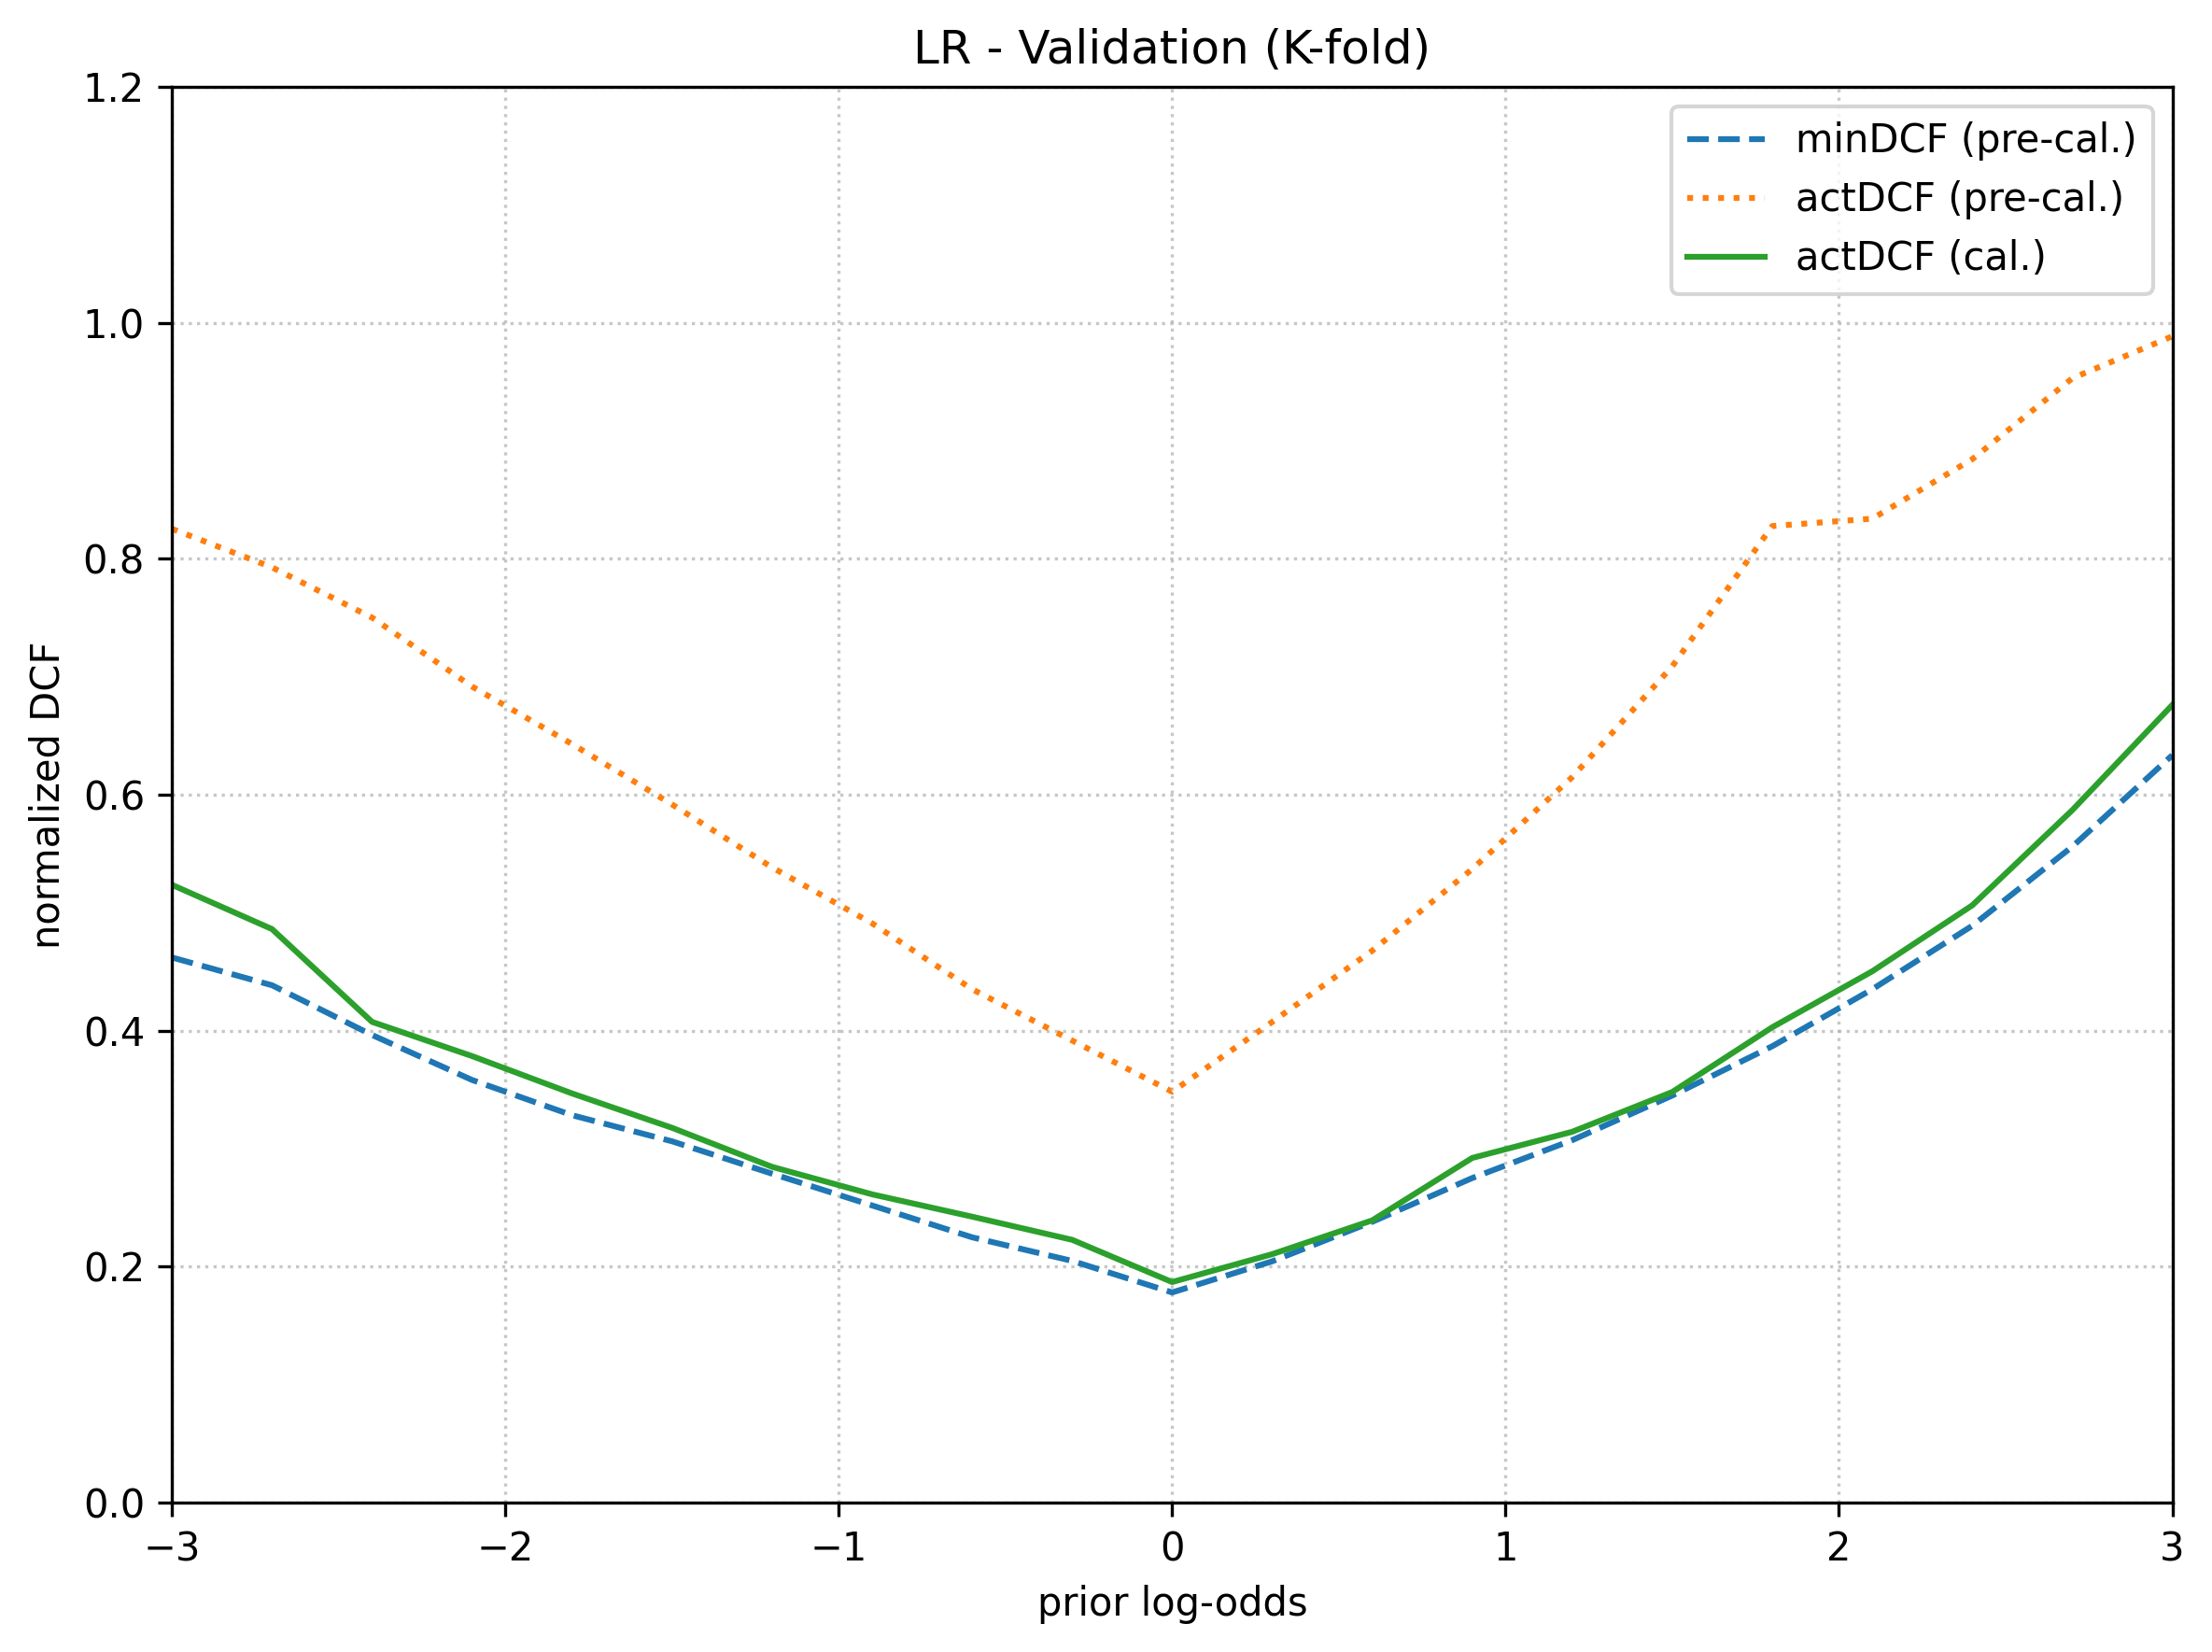
\includegraphics[width=\linewidth]{LR_kfold_val.png}
\caption{Calibrated Bayes Error: Logistic Regression.}
\label{fig:cal_lr}
\end{minipage}\hfill
\begin{minipage}{0.48\textwidth}
\centering
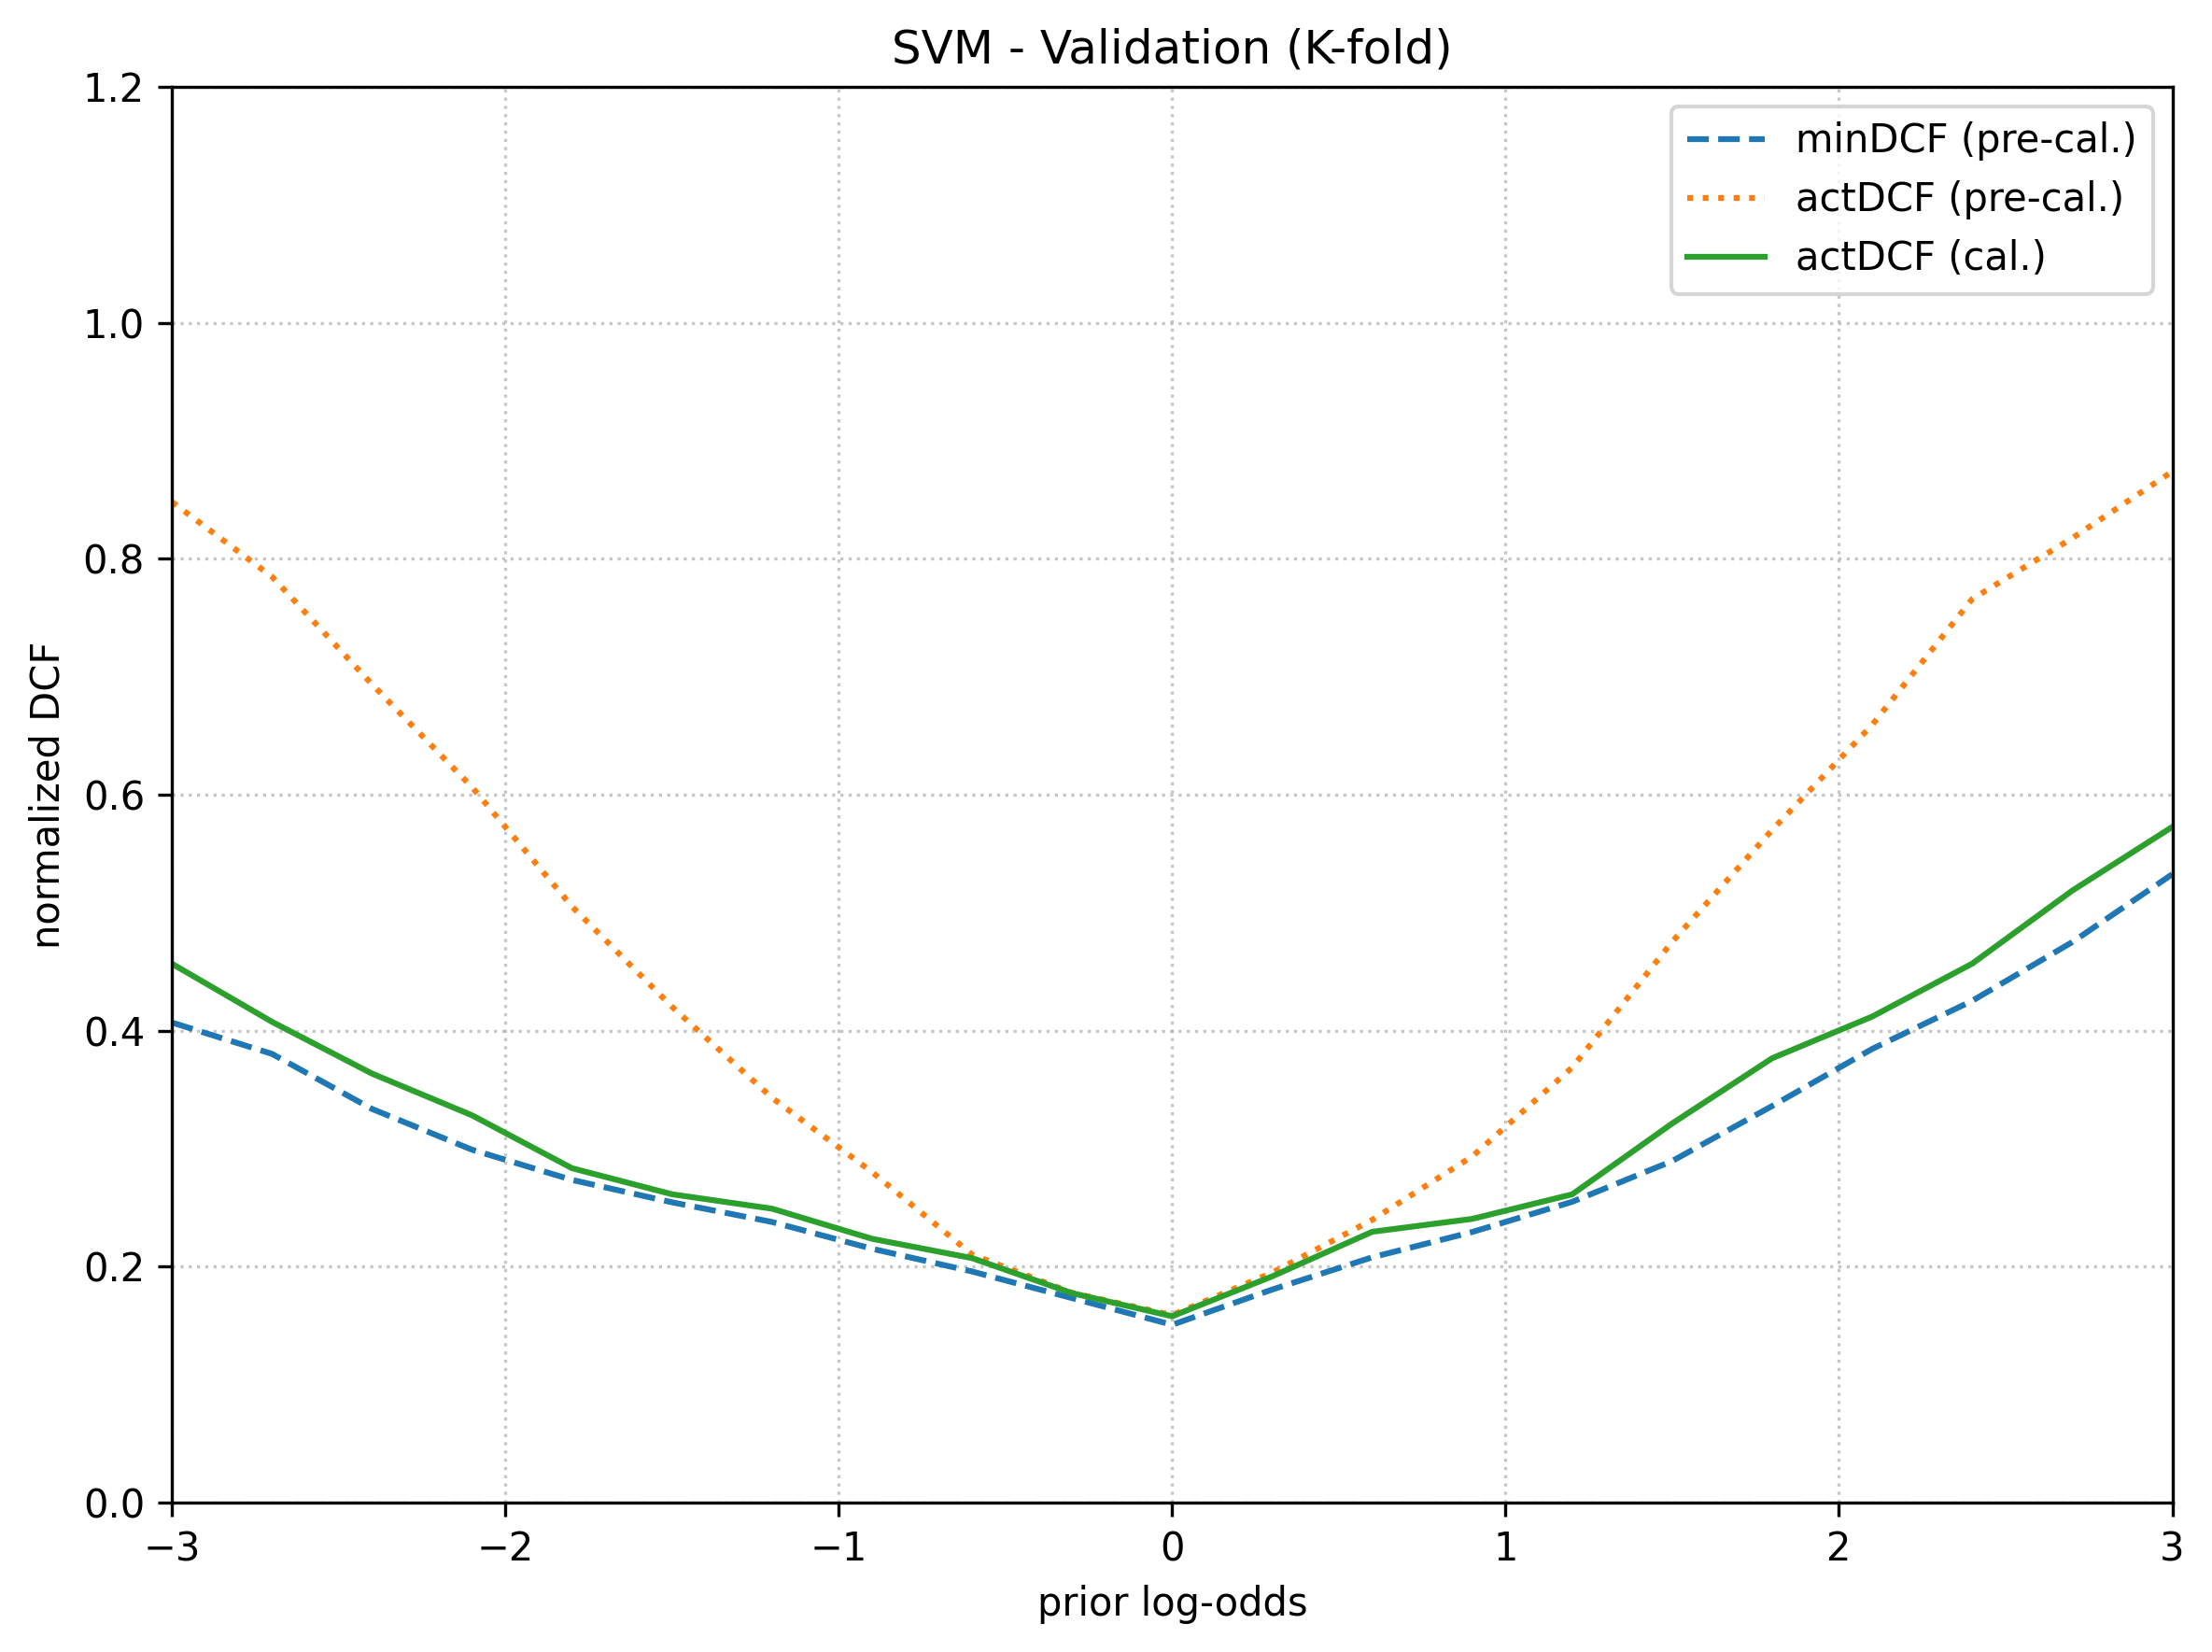
\includegraphics[width=\linewidth]{SVM_kfold_val.png}
\caption{Calibrated Bayes Error: SVM (RBF).}
\label{fig:cal_svm}
\end{minipage}
\end{figure}
\begin{figure}[H]
\centering
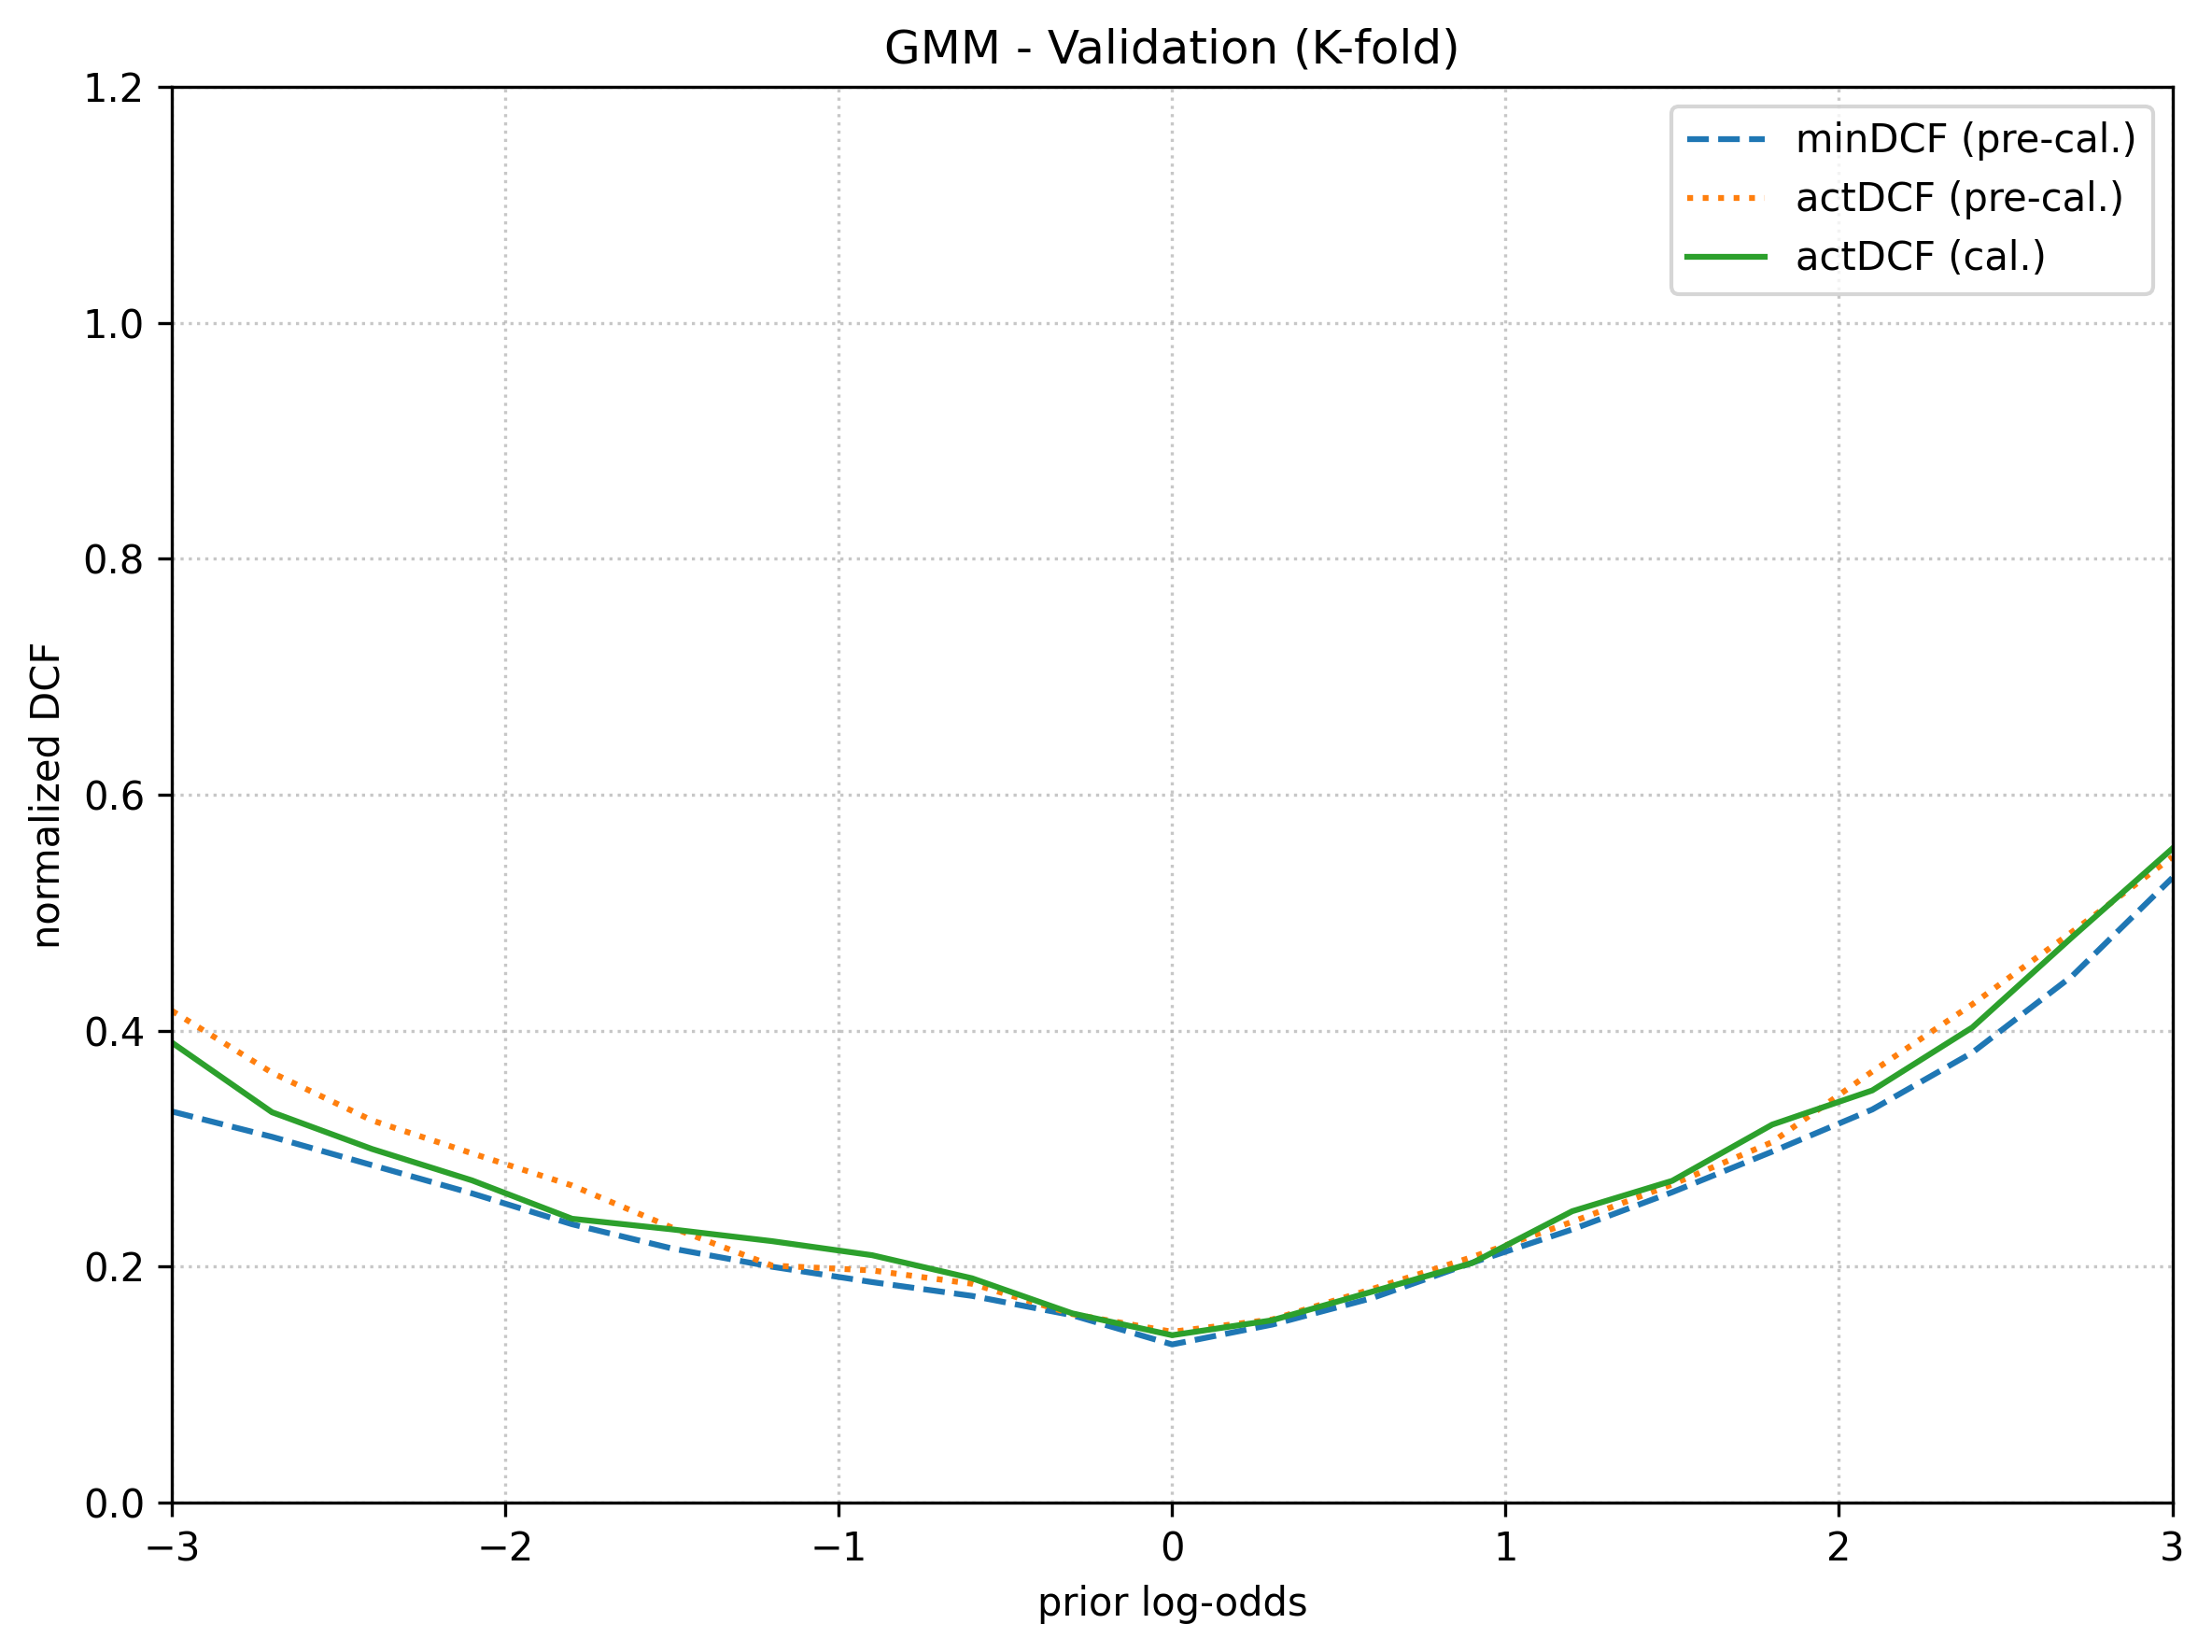
\includegraphics[width=0.5\textwidth]{GMM_kfold_val.png}
\caption{Calibrated Bayes Error: Tied GMM.}
\label{fig:cal_gmm}
\end{figure}
\subsection*{Question: What do you observe from the Bayes error plots?}
Observing the Bayes Error plots for the calibrated scores, the most prominent feature is the near-total elimination of the divergent "trumpet shape" at the extreme log-odds.
In the uncalibrated models evaluated previously, the Actual DCF (red curve) lifted significantly away from the Minimum DCF (blue curve) as the prior log-odds moved away from 0. In these calibrated plots, the Actual DCF curve closely hugs the Minimum DCF curve across the entire spectrum from -4 to +4. While a marginal gap remains at the absolute extremes (particularly for Logistic Regression), the overall geometric profile confirms that the output scores have been successfully restructured to function as highly accurate log-likelihood ratios.
\subsection*{Question: Was the calibration strategy effective for the different approaches?}
Yes, the calibration strategy was highly effective, though the magnitude of its impact varied drastically depending on the underlying architecture:
\begin{itemize}
\item \textbf{Support Vector Machine (SVM):} The calibration was overwhelmingly effective. At $\tilde{\pi}=$0.1, the Actual DCF plummeted from a severely miscalibrated 0.631 down to 0.347. At $\tilde{\pi}=$0.9, it dropped from 0.694 to 0.411. The calibration process rescued the SVM from being entirely unusable at extreme priors.
\item \textbf{Gaussian Mixture Model (GMM):} The calibration was effective but provided a more modest refinement. Because the GMM natively outputs probabilistic log-likelihoods, its raw scores were already reasonably scaled. Still, calibration successfully closed the gap at $\tilde{\pi}=$0.1, reducing the Actual DCF from 0.303 to 0.279.
\item \textbf{Logistic Regression:} Calibration successfully mitigated the structural bias introduced by its original training prior ($p_T=0.5$). For instance, at $\tilde{\pi}=$0.1, the Actual DCF improved from 0.413 to 0.387.
\end{itemize}
\section{Theoretical Considerations}
The profound success of the score calibration—particularly for the Support Vector Machine—can be explained by the mathematical mechanics of the affine transformation applied by the Logistic Regression calibrator.
Calibration seeks to find a mapping $s_{cal} = \alpha s + \beta - \log \frac{\tilde{\pi}}{1-\tilde{\pi}}$ such that the shifted scores directly represent the true empirical log-odds of the classes.
As established in Chapter 1, the SVM is a non-probabilistic, margin-maximizing model. Its raw scores s represent the geometric distance from the separating hyperplane in the RBF-induced feature space. These distances are boundless and do not naturally scale alongside Bayesian probability thresholds. The Logistic Regression calibrator effectively acts as a sigmoid squashing function (Platt Scaling), discovering the optimal slope ($\alpha$) and bias ($\beta$) to warp these geometric distances into properly scaled probabilities. This is why the SVM saw the most dramatic recovery in its Actual DCF.
For the generative GMM, the calibration serves a different theoretical purpose. While the GMM already outputs log-likelihoods, those likelihoods are mathematically rigid, assuming the data strictly adheres to the mixture components. As we discovered in Laboratory 4, Features 5 and 6 exhibit heavy skewness that violates ideal Gaussian assumptions. The calibrator acts as a final error-correction layer, linearly adjusting the GMM's density estimates to compensate for the slight probabilistic distortions caused by the non-Gaussian tails of the true data distribution.